\section{Methods}
\label{sect:methods}  % \label{} allows reference to this 

To assess the viability of GBD for high-contrast imaging simulation we first compare the point-spread function (PSF) produced by GBD to one produced by an equivalent Fresnel diffraction model for a given observatory. This comparison is done to assess the ability of GBD to achieve Fresnel-equivalent performance using the same assumptions. The Fresnel model is built with the open-source package POPPY (Physical Optics Propagation in PYthon), which was developed to simulate the PSFs of the James Webb Space Telescope\cite{Perrin12}. Fresnel diffraction represents the state of the art for coronagraph modeling because of the method's capacity to model near-field effects that limit high-contrast imaging (e.g. the Talbot effect\cite{goodman17}). Our GBD module's capacity to model Fresnel-equivalent phenomena\cite{Ashcraft2020} has been illustrated in a previous investigation, so we now investigate its feasibility to produce an accurate model of an observatory's PSF. In this section we illustrate the operating principles of Gaussian beam propagation and how they are used to simulate arbitrary fields.

% POPPY has been verified against PROPER\cite{krist_2007} and is used to simulate the Roman Space Telescope Coronagraph Instrument (ROMAN-CGI)\cite{Milani2021}. 

\subsection{Gaussian Beam Parameters}
To propagate an arbitrary optical beam the field must be decomposed into a finite sum of Gaussian beamlets which are then independently propagated. A single Gaussian Beam is described entirely by the complex beam parameter $q(z)$: \cite{goodman17}
\begin{equation}
	U(r,z) = \frac{U_o}{q(z)}exp[ik\frac{r^2}{2q(z)}]
\end{equation}

Where $U_o$ is the amplitude, $k$ is the wavenumber, and $r$ is the radial coordinate in the plane perpendicular to propagation. The complex parameter $q(z)$ describes the beam's $1/e$ field size (the "waist" $w_o$) and wavefront radius of curvature $R(z)$. 
\begin{equation}
	q(z)^{-1} = \frac{1}{R(z)}+i\frac{\lambda}{\pi w(z)^2}
\end{equation}	
$q(z)$ is a convenient expression of the Gaussian beam because it fully encapsulates the information required to describe the transverse electric field of the beam as it propagates. The real part of $q(z)$ is related to the radius of curvature of the wavefront.
\begin{equation}
	R(z) = z(1+(\frac{Z_o}{z})^2)
\end{equation}
Where $Z_o$ is the Rayleigh range and $z$ is the longitudinal propagation distance.
The imaginary part of $q(z)$ is related to the beam waist radius
\begin{equation}
	w(z) = w_o\sqrt{1+(\frac{z}{Z_o})^2}
\end{equation}
In the paraxial regime $q(z)$ can be propagated using the ABCD ray transfer matrices of geometrical optics.
\begin{equation}
    q(z)^{-1}_{o} = \frac{C + D/q_{i}}{A + B/q_{i}}
\end{equation}
For the generally astigmatic case, $q(z)$ is a 2x2 matrix $\textbf{Q}(z)$ that encodes the complex curvature in two orthogonal directions and how they couple into each other\cite{Ashcraft2020,cai_decentered_nodate}. 

\begin{equation}
    \textbf{Q}(z)^{-1} = 
    \begin{pmatrix}
    q(z)_{xx}^{-1} & q(z)_{xy}^{-1} \\
    q(z)_{yx}^{-1} & q(z)_{yy}^{-1} \\
    \end{pmatrix}
\end{equation}

This treatment allows for greater versatility in the beamlet propagation, but requires that the elements of the ray transfer matrices are also 2x2 matrices. The propagation of the generally decentered and astigmatic Gaussian beam is described in Cai and Lin\cite{cai_decentered_nodate}, which derives an expression of the beam propagation purely in terms of matrix optics. By leveraging this unique parameter of the Gaussian beam we can perform diffraction calculations without traditional Fourier-transform based methods. The full equation in matrix form is given in equation \ref{eq:DEGB}.

\begin{equation}
    U(\vec{r}_{o}) = \frac{e^{ikl_{o}}}{|\mathbf{A} + \mathbf{BQ_{1}^{-1}}|^{1/2}} e^{-\frac{ik}{2}\vec{r_{o}}^{T}\mathbf{Q_{2}}^{-1}\vec{r_{o}}} e^{-\frac{ik}{2}\vec{r_{i}}^{T}(\mathbf{Q_{1}}^{-1} + \mathbf{A}^{-1}\mathbf{B})\vec{r_{i}}} e^{ik\vec{r_{i}}^{T}(\mathbf{A}\mathbf{Q_{1}}^{-1} + \mathbf{B})\vec{r_{o}}}
    \label{eq:DEGB}
\end{equation}

Note that the arguments of the exponential are scalar valued quantities, and are represented in matrix form for brevity.

\subsection{Entrance Pupil Spatial Decomposition}

The operating principle of GBD is to decompose the field in the optical system's entrance pupil into a finite sum of Gaussian beamlets. Our module spatially decomposes the field at the entrance pupil and propagates each beamlet along a ray path using equation \ref{eq:DEGB}. Various sample schemes exist in the literature, with different strengths and weaknesses. The "even" sample scheme described in Harvey et al\cite{Harvey15} is the most straightforward, where the beamlets lie evenly spaced along a square grid. The ray coordinates in the entrance pupil are then computed from an overlap factor (OF) which describes the overlap of the beamlets $1/e$ waist radii $w_o$\cite{Worku:18}.

\begin{equation}
    OF = \frac{N_{g} 2 \omega_{o}}{W}
\end{equation}

Where $N_{g}$ is the number of Gaussian beamlets across an aperture, and $W$ is the width of the aperture. This feature is easy to implement and understand, but for under-sampled cases it introduces artifacts due to the ripple and soft edge left by the Gaussian beamlets. The "Fibonacci" sample scheme introduced by Worku and Gross \cite{Worku:18} places the beamlets along a Fibonacci spiral such that the RMS error of the decomposed field is minimized. Hexapolar sampling is also a viable method to increase the accuracy of the decomposition for fewer beamlets assuming the optical system has a circular aperture\cite{Worku:18}. Both sample schemes are not well-matched to Cartesian grids, so applying wavefront error arrays to optical elements requires interpolation of the surface, which slows the simulation. For the results presented in this paper, we employ the even sample scheme.


% y-axis is RMS error to a tophat
% W is fixed
% wo is fixed
% OF is variable, which changes the number of gaussians
% \begin{figure}[H]
%     \centering
%     \includegraphics{}
%     \caption{RMS error to a tophat beam v.s. OF and beam waist for a set number of Gaussian beamlets. }
%     \label{fig:sampleschemes}
% \end{figure}


\subsection{Paraxial Model w/ Arbitrary WFE}

First we construct a paraxial model of the observatory to compare GBD against Fresnel diffraction for modeling astronomical observatories and their coronagraphs. The paraxial model carries the same assumptions of Fresnel diffraction: that the angles are small and that all optics are gaussian  reduced to their principal planes\cite{goodman17}. This comparison will show that GBD is suitable to mimicing the performance of Fresnel diffraction-based propagators. In the paraxial assumption ray propagation is handled by ray transfer matrices for propagation ($\textbf{D}$) and refraction ($\textbf{L}$)\cite{Ashcraft2020} 

\begin{equation}
    \mathbf{L} = 
    \begin{pmatrix}
    1 & 0 & 0 & 0 \\
    0 & 1 & 0 & 0 \\
    -1/f_x & 0 & 1 & 0 \\
    0 & -1/f_y & 0 & 1 \\
    \end{pmatrix}
    ;                
    \mathbf{D} = 
    \begin{pmatrix}
    1 & 0 & d/n & 0 \\
    0 & 1 & 0 & d/n \\
    0 & 0 & 1 & 0 \\
    0 & 0 & 0 & 1 \\
    \end{pmatrix}
\end{equation}

Where $\mathbf{L}$ is the matrix representing a thin lens of focal length $f$ and $\mathbf{D}$ is the matrix representing the propagation of rays by a distance $d$. The generally nonorthogonal optical system permits propagation through optics with focal lengths that are not equal in $x$ and $y$, but for the paraxial model all lenses are set such that $f_x = f_y$. Constructing an optical system with these matrices is done by taking their matrix product.

\begin{equation}
    \mathbf{O_{sys}} = \prod_{i = 1}^{N} \mathbf{D}_{i} \mathbf{L}_{i}
\end{equation}

Where a general optical system can be reduced to $N$ interactions of a refraction by the $i$-th optic $\textbf{L}_{i}$ and propagation by the $i$-th distance $\textbf{D}_{i}$.

Low-order aberrations are of importance to the design of coronagraphs for observatories because they spread the PSF over the focal plane mask which couples starlight into the high-contrast region of the coronagraph. Consequently tracing the low-order aberrations accurately is of paramount importance to any propagation physics used for high-contrast imaging modeling. In the paraxial regime, we model wavefront errors on optics with Jeong et al's arbitrary wavefront error ray transfer matrix\cite{Jeong:05}. For a given optical path difference $W(x,y)$ the nonorthogonal ray transfer matrix can be computed by calculating the gradient of the wavefront error function.

\begin{equation}
    \mathbf{W}(x,y) = 
    \begin{pmatrix}
    1 & 0 & 0 & 0 \\
    0 & 1 & 0 & 0 \\
    \frac{1}{x}\frac{\partial W(x,y)}{\partial x}& 0 & 1 & 0 \\
    0 & \frac{1}{y}\frac{\partial W(x,y)}{\partial y} & 0 & 1 \\
    \end{pmatrix}
\end{equation}

Where $x,y$ are the coordinates of the ray incident on the surface with wavefront error $W$. Jeong et al showed the analytical computations of wavefront error as a sum of Zernike polynomials, but in this investigation we used numpy's gradient function to compute the wavefront error for any arbitrary array. Doing this decreases the number of matrix products needed to describe the optical system. However, each ray path must encounter a different ray transfer matrix for derivatives of $W$ that are not constant. The effective paraxial optical system is given by $\mathbf{O}_{paraxial}$

\begin{equation}
    \mathbf{O}_{paraxial} = \mathbf{D}\mathbf{L}\mathbf{W}
\end{equation}

Such that the wavefront is aberrated, focused, and then propagated to the image plane. This investigation will simply evaluate GBD in the case where it is trying to employ the same assumptions as Fresnel diffraction with entirely different physics, without the benefits of modeling non-paraxial effects. 

\subsection{Nonparaxial Model with Differential Ray Tracing}

The key benefit of using GBD for observatory modeling is its ability to model the PSF of an observatory using ray data. The paraxial assumption is only made along a single raypath, so coherent calculations can be done for generally nonparaxial systems. However, to use Cai and Lin's equation to propagate the beamlet the ray transfer matrix must be solved for every ray in the optical system. To do so we implement differential ray tracing to solve the matrix in terms of the derivatives of the ray data. Differential ray tracing is a key tool in optical design software used in a variety of applications \cite{Stone:97,stone_tech_memo}. We employ this technique by using a ray tracing engine (Zemax OpticStudio) that propagates rays by computing Snell's Law at each surface. A local coordinate system is defined for both the input and output surface, and the ray derivatives are computed using the finite differences method. An example of computing the element $A_{x,x}$ is given by equation \ref{eq:Axx}. In this example two rays are traced, one with a differential addition in input $x$ coordinate and one with no change. The $x$ coordinates of these input and output rays determine the derivative. 

\begin{equation}
    A_{xx} = \frac{\partial x_{2}}{\partial x_{1}} = \frac{x_{output,+x} - x_{output,o}}{x_{input,+x} - x_{input,o}}
    \label{eq:Axx}
\end{equation}

The ray transfer matrix for a non-orthogonal optical system has 16 unknowns, and each ray yields 4 quantities. To solve for every element of the matrix 4 linearly independent rays must be traced. The simplest ray set is geometrically orthogonal\cite{Greynolds86}, where copies of the central ray $(x,y,u,v)$ are modified by a differential quantity $(\delta)$ in each of the 4 ray coordinates.

\begin{center}
    
\begin{equation}
    \begin{pmatrix}
    x + \delta x \\
    y \\
    u \\
    v \\
    \end{pmatrix}
    ,
    \begin{pmatrix}
    x \\
    y + \delta y \\
    u \\
    v \\
    \end{pmatrix}
    ,
    \begin{pmatrix}
    x \\
    y \\
    u + \delta u\\
    v \\
    \end{pmatrix}
    ,
    \begin{pmatrix}
    x \\
    y \\
    u \\
    v + \delta v\\
    \end{pmatrix}
\end{equation}

\end{center}
The ray of interest is propagated along with four rays that enable the computation of the local derivatives in position ($x,y$) and angle ($u,v$). The full differential ray transfer matrix is given by equation \ref{eq:diffmat}. The ray transfer matrix is purely a function of the Cartesian position of the ray ($x,y$) and  slope of the ray in those directions ($u,v$) at the input and output of the optical system.

\begin{figure}[H]
    \centering
    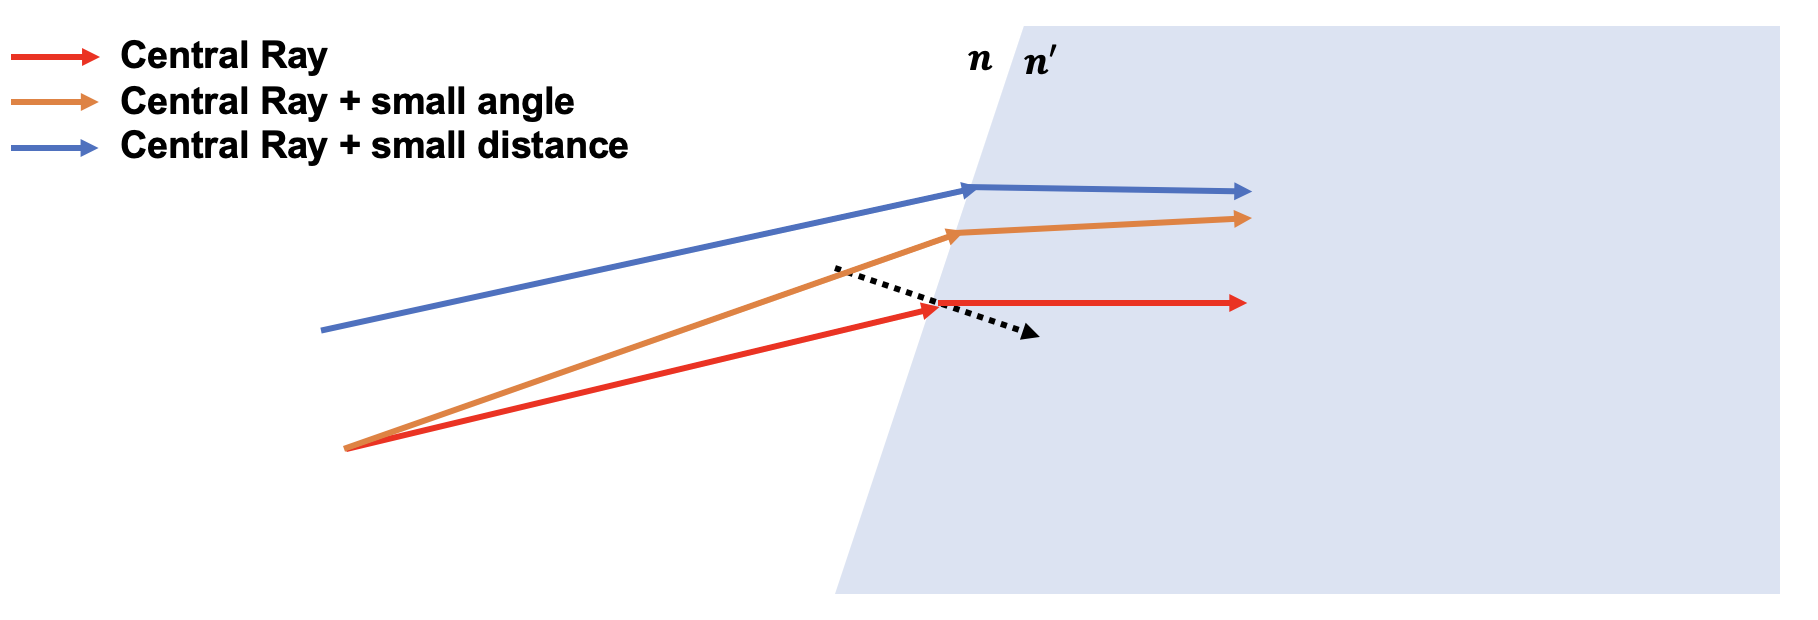
\includegraphics[width=\textwidth]{differential_diagram.png}
    \caption{Diagram illustrating differential ray tracing in the 2D case on a locally planar interface between media with incident refractive index $n$ and transmitted refractive index $n'$. The black dotted line indicates the surface normal for the interaction with the central ray.}
    \label{fig:my_label}
\end{figure}


\begin{center}
    
\begin{equation}
    \begin{pmatrix}
    x' & y' & u' & v' \\
    \end{pmatrix}
    =
    \begin{pmatrix}
    \frac{\partial x_2}{\partial x_1} & \frac{\partial x_2}{\partial y_1} & \frac{\partial x_2}{\partial u_1} & \frac{\partial x_2}{\partial v_1}  \\
    \frac{\partial y_2}{\partial x_1} & \frac{\partial y_2}{\partial y_1} & \frac{\partial y_2}{\partial u_1} & \frac{\partial y_2}{\partial v_1}  \\
    \frac{\partial u_2}{\partial x_1} & \frac{\partial u_2}{\partial y_1} & \frac{\partial u_2}{\partial u_1} & \frac{\partial u_2}{\partial v_1} \\
    \frac{\partial v_2}{\partial x_1} & \frac{\partial v_2}{\partial y_1} & \frac{\partial v_2}{\partial u_1} & \frac{\partial v_2}{\partial v_1} \\
    \end{pmatrix}
    \begin{pmatrix}
    x \\
    y \\
    u \\
    v \\
    \end{pmatrix}
    %$
    \label{eq:diffmat}
\end{equation}

\end{center}
Because Gaussian beamlets are propagated along geometric ray paths, computing the differential ray transfer matrix enables the propagation of a beamlet through an arbitrary optical system. Using this matrix any open-source diffraction model can be linked to a ray trace model of an observatory.

\subsection{Accelerated Computing}

%The propagation of the beamlets from the entrance pupil to the plane of interest is fast because it is done with ray tracing. However, a known limitation of GBD is the time taken to enable a highly sampled simulation\cite{Ashcraft2020} using Python's numpy to compute the exponential for a very large number of beamlets. In contrast, FFT-based diffraction models are computationally faster for a single element, but the computation time is slowed by the number of elements in the system due to the increase in FFT operations needed.

The independence of the Gaussian beamlet operations are uniquely suited to the exploration of multi-threaded computation to accelerate diffraction simulations. Accelerated computing is integral to diffraction modeling to enable rapid and precision simulation of small signals. 
The time to conduct traditional Fourier-based diffraction modeling is set by the complexity of the system. The sampling of each optical element and the number of total optical elements increase the complexity and number of Fast Fourier Transforms (FFT) used, resulting in more computation time. GBD circumvents the FFT entirely by tracing rays to propagate through the optical system in a fraction of the time of the FFT. GBD’s diffraction calculation at the plane of interest computes an exponential of an array that scales with the number of beamlets and sampling of the image plane, resulting in longer computation times.  Preliminary explorations into accelerated computing were conducted using the numexpr\cite{numexpr} and numba\cite{lam_numba_2015} Python packages that showed favorable computation time decreases by multi-threading the operation on a CPU. Both packages operate by pre-compiling a given function into machine code that the program calls and breaking up the operation into chunks of arrays that a CPU core can handle efficiently. The key computational advantage of GBD is the ability to do diffraction calculations in parallel. Numba was the first package explored due to its ease of implementation. The package works by applying a decorator to a Python function that processes the large array of interest, and then specifying the number of central processing unit (CPU) cores for the process to use. The distribution of the information stored within the array is handled automatically by numba, and results in considerable runtime decreases for GBD. On a 16 core 2.4GHz CPU, runtime for a simulation of 1876 Gaussian beamlets through a coronagraph to simulate a 256x256 pixel focal plane was sped up by a factor of 5, which approached POPPY's Fresnel diffraction runtime. This experiment was repeated using the numexpr package which showed an even greater decrease in computation time. The comparison in runtime vs. number of CPU cores is shown in Fig. 6.

\begin{figure}[H]
    \centering
    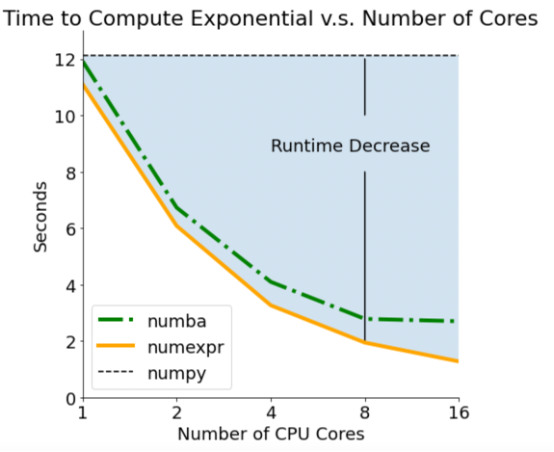
\includegraphics[width=0.6\textwidth]{runtime.png}
    \caption{Run time comparison for a 50x50 grid of Gaussian beamlets on a 256 x 256 detector grid v.s. number of CPU cores used. }
    \label{fig:runtime_sim}
\end{figure}

We anticipate even greater speedups on graphical processing units (GPU), and intend to add GPU compatibility to our GBD module in future work.